\phantomsection

\chapter{Desenvolvimento}

O presente capítulo é dividido em duas fases, a primeira apresenta o desenvolvimento e os resultados das etapas da metodologia de desenvolvimento do protótipo do dispositivo.
E a segunda seção apresenta a metodologia do experimento utilizado como prova de conceito do dispositivo desenvolvido.

Como visto na seção de introdução é observado que existem diversas limitações e dificuldades no sensoriamento de cargas de torque em eixos, este trabalho é tem como objetido
desenvolver uma solução para tal problema assim criando uma alternativa que facilita o acesso e diminui os custos para a obtenção desses tipos de dados.

Um dispositivo existente que é utilizado para obter dado de cargas de torção são os transdutores de torque, que são são dispositivos que tem como princípio de funcionamento
a utilização de um sensor de deformação em um eixo de dimensões conhecidas que se encontra sob a atuação das cargas, esses dispositivos são utilizados em aplicações de experimento
ou industriais.
Os sinais de tensão obtidos são transferidos em tempo real utilizando contatos elétricos rotativos \autocite{Kyowa}.
A utilização de um transdutor de torque em uma aplicação industrial é mostrada na \autoref{fig:2001}.

\begin{figure}[htb]
	\caption{\label{fig:2001} Utilização de um transdutor de torque}
	\begin{center}
		\includegraphics[width=\textwidth]{pictures/2001.png}
	\end{center}
	\fonte{\autocite{Kyowa}}
\end{figure}

Será desenvolvido um dispositivo baseado no funcionamento do transdutor de torque apresentado, porém, ao invés da transmissão de dados via contato elétrico rotativo será
desenvolvido um conceito em que os dados são transmitidos via conexão sem fio, com o objetivo de se criar um produto que funcione de maneira totalmente remota sem a necessidade
de utilização de nenhum chicote para a transmissão dos dados.

\section{Planejamento do projeto}

A primeira etapa para realizar o planejamento do projeto foi uma pesquisa de custo e disponibilidade de produtos iguais ou semelhantes a este propósito no mercado digital,
os resultados da pesquisa são apresentados na próxima subseção.

\subsection{Mapeamento tecnológico}

Foram encontrados inúmeros dispositivos para telemetria e obtenção de sinais de sensores para aplicações industriais, no mapeamento foram considerados apenas os que foram
encontrados a preços acessíveis.
Dos produtos encontrados, dois se mostraram de grande semelhança ao conceito que será desenvolvido.

A empresa Isso disponibiliza em sua loja virtual um dispositivo para controle e obtenção de dados, denominados dmi tcr 44es, mostrado na \autoref{fig:2010}.
Segundo o fabricante esse dispositivos é utilizado para aplicações de acionamentos e telemetria remota, e é indicados para uso em automações residenciais e
industriais \autocite{Isso44es}.
A empresa também disponibiliza outro modelo muito semelhante, denominado dmi tcr 88es, que possui maior número de conexões de entradas e saídas de sinais.

\begin{figure}[htb]
	\caption{\label{fig:2010} Datalogger DMI TCR 44es}
	\begin{center}
		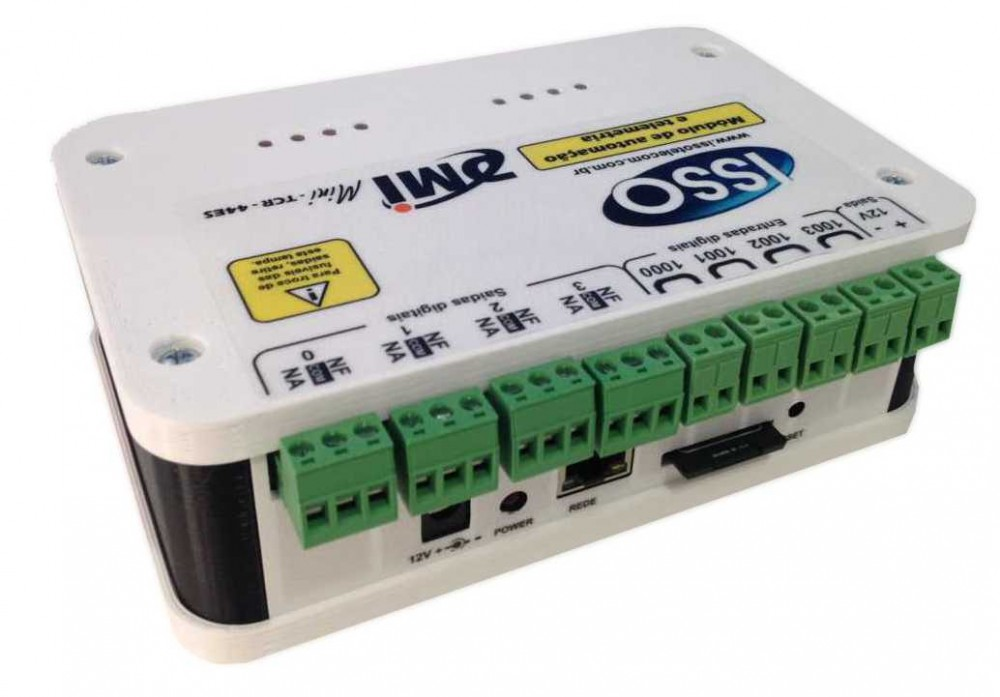
\includegraphics[width=\textwidth]{pictures/2010.jpg}
	\end{center}
	\fonte{\autocite{Isso44es}}
\end{figure}

Outro dispositivo, denominado Bridge101A, mostrado na \autoref{fig:2030}, fabricado pela empresa Madgetech foi encontrado.
Segundo o fabricante é um dispositivo de obtenção de dados compacto que mede e armazena valores de tensões elétricas, e é normalmente utilizado com extensômetros, células
de carga e outros sensores de baixa tensão, e é utilizado para calcular com precisão parâmetros de tensão, torque, deformação e pressão ao longo do tempo \autocite{Bridge101A}.

\begin{figure}[htb]
	\caption{\label{fig:2030} Dispositivo Bridge101A}
	\begin{center}
		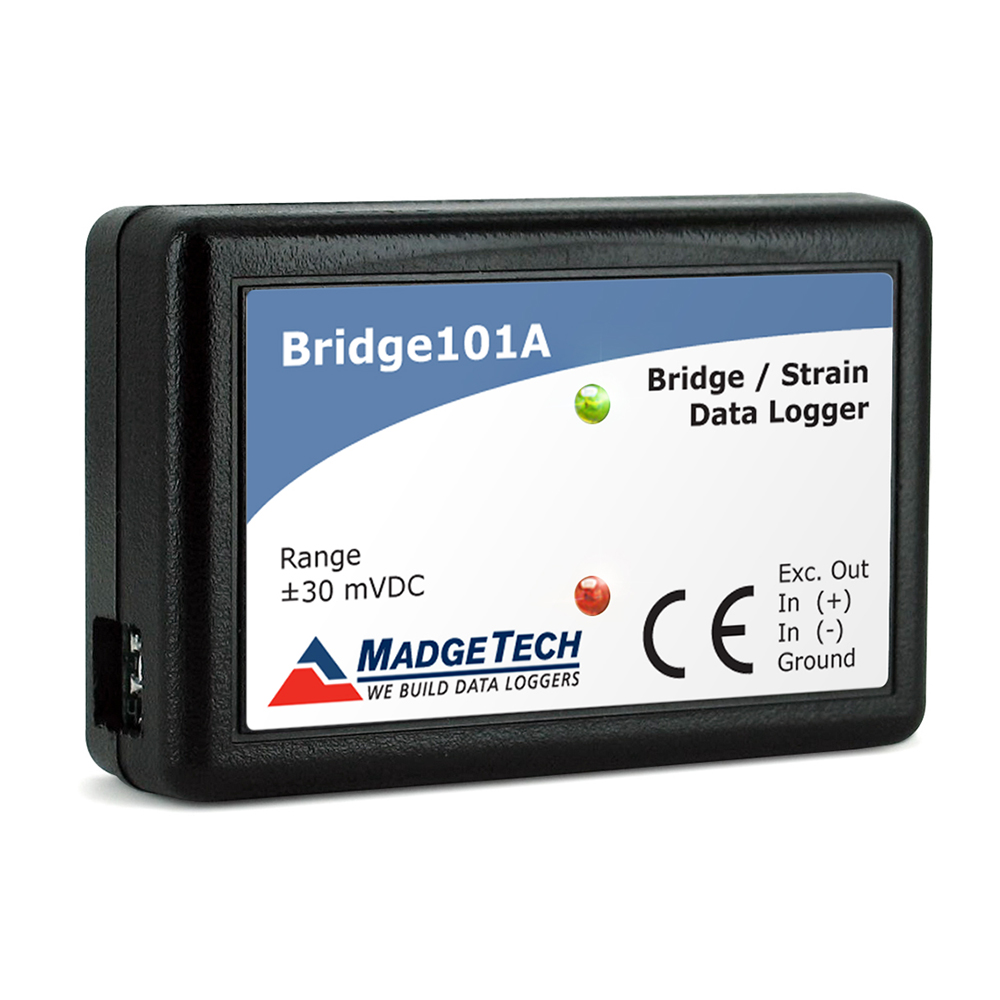
\includegraphics[width=\textwidth]{pictures/2030.jpg}
	\end{center}
	\fonte{\autocite{Bridge101A}}
\end{figure}

A \autoref{tab:Banchmarking} mostra uma comparação entre os dados de utilização obtidos pela documentação dos dois dispositivos previamente apresentados.

\begin{table}[!ht]
    \caption{Comparação entre dispositivos encontrados}
    \label{tab:Banchmarking}
    \centering
    \resizebox{\linewidth}{!}{%
        \begin{tabular}{ l | c c r } \toprule
         			  & Isso DMI TCR 44es & Isso DMI TCR 88es & Madgetech Bridge101A \\
			\midrule
			Dimensões & 124x117x55mm & 190x117x55mm & 36x64x16mm \\
			Comunicação com PC & Conexão Ethernet & Conexão Ethernet & Conexão USB \\
%			Interface com o usuário & Software próprio & Software próprio & Software próprio \\
%			Programação & Software próprio & Software próprio & Software próprio \\
			Taxa de leitura & Não disponiblizado & Não disponiblizado & $\SI{4}hz$ \\
			Faixa de tensão de leitura & Não disponiblizado & Não disponiblizado & $\SI{\pm 30}{\mV}$ \\
			Faixa de preço & R\$1100,00 & R\$1300,00 & R\$2800,00 \\
            \bottomrule
        \end{tabular}}
\fonte{O autor 2022}
\end{table}

Dentre os valores apresentados na tabela fica claro os altos preços envolvidos em qualquer aplicação que necessite a utilização desse tipo de dispositivo.
Muitos deles adicionalmente necessitam de softwares proprietários pagos para sua programação e utilização.
O dispositivo desenvolvido neste trabalho tem como objetivo um preço consideravelmente menor que os analisados e programável e utilizável utilizando tecnologias
de código aberto.

\subsection{Pesquisa científica}

Com o intuito de facilitar o desenvolvimento do dispositivo, foi realizada uma revisão sistemática de trabalhos científicos e acadêmicos disponíveis nas bases de dados Web of Science, Springer,
Sciencedirect e Google Scholar, utilizando como palavras-chave “Dynamic, Torque, Shaft, Sensor, Strain, Gauge”, os principais obtidos são apresentados nessa subseção.

Um artigo desenvolvido por Niedworok relata o desenvolvimento e aplicação de um sistema de sensoriamento de torque em tempo real em um eixo cardã de um carro de mina
utilizando a medição da deformação utilizando extensômetro com transferência dos dados via radiofrequência.
O trabalho também indica que o posicionamento do sensor necessita estar em contato com a superfície de maior deformação do componente, o autor realiza uma análise por elementos finitos
para encontrar esse local.
O artigo também aponta que o sinal vindo do sensor deve ser ampliado utilizando uma ponte de Wheatstone para conseguir ter a instrumentação correta da grandeza.
O artigo mostrou resultados satisfatórios e não discutiu sobre ruídos e imprecisões presentes nos dados obtidos. \autocite{Niedworok2014}

Nurprasetio desenvolve, em seu trabalho, um sistema de medição para veículos terrestres, aplicado em uma bancada de testes que simula o estado de veículos terrestres em operação, o sistema
utiliza um microprocessador Arduino nano de fácil acesso e baixo custo, em que s dados são transmitidos via comunicação bluetooth.
O artigo também ilustra o processo de calibração do dispositivo feito antes do teste dinâmico, assim como no trabalho anterior, também é enfatizada a necessidade das metodologias de instrumentação
do sinal vindo do extensômetro.
Seus resultados também se mostraram promissores, porém o autor indica que é necessário a remoção dos ruídos de medição, o que segundo ele será endereçado em um trabalho futuro \autocite{Nurprasetio2018}.

Gharghan compara um sistema de medição similar ao dos dois trabalhos prévios com um sistema de medição de torque em tempo real de alto custo utilizado por ciclistas profissionais no pedivela.
O artigo introduz a tecnologia de transmissão de dados Zigbee, que consegue transmitir dados a um baixo consumo energético.
Após a obtenção dos dados, o autor utiliza as ferramentas de análise estatística de Bland-Altman obtendo a porcentagem de erro médio absoluto para a validação do sistema \autocite{Gharghan2017}.

Silva compara os dados de um sistema semelhante aos anteriores com resultados de análises de modelo matemático analítico e análise por elementos finitos aplicados em bancadas de viga engastada com carga
na ponta e de torque aplicado em um eixo com um dos lados travados, diferente dos trabalhos anteriores, este possui uma seção com o desenvolvimento das equações dos modelos utilizados, e assim como os artigos
anteriores foram encontrados resultados satisfatórios \autocite{Silva2017}.

A ideia inicial da concepção do produto seria o do desenvolvimento de um dispositivo que obtivesse os valores de torque em um eixo em tempo real.
Para que fosse possível solucionar tal problema, o dispositivo teria que obter os dados de tensão dos polos de uma ponte de wheatstone, com um extensômetro montado a um eixo sob torque e transmitir os dados obtidos
via conexão sem fio em tempo real a um computador.

A modelagem de um produto conceito inicial baseado nos resultados da pesquisa de mercado e nos trabalhos científicos foi elaborado pelo autor utilizando o software Solidworks 2017,
esta modelagem é mostrada na \autoref{fig:2029}.

\begin{figure}[htb]
	\caption{\label{fig:2029} Projeto inicial do dispositivo}
	\begin{center}
		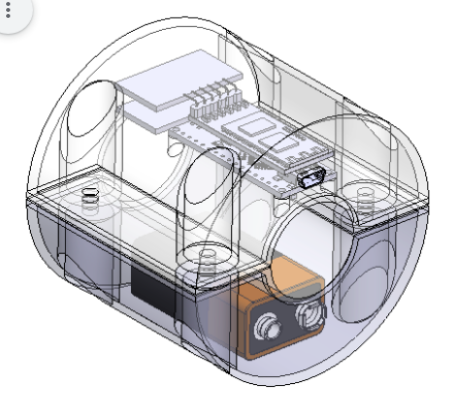
\includegraphics[width=\textwidth]{pictures/2029.png}
	\end{center}
	\fonte{O autor 2022}
\end{figure}

O conceito é composto por uma placa de desenvolvimento Arduino nano, que controla um amplificador de sinal que por si obtém os dados de tensão de uma ponte de wheatstone.
Os dados obtidos pela ponte de wheatstone então são transmitidos utilizando um módulo bluetooth HC-05.
O custo total desses dois componentes é baixo, e um protótipo de dispositivo pode ser montado por aproximadamente $R\$150,00$, desconsiderando os componentes de encapsulamento.
O projeto informacional é iniciado considerando este conceito como a ideia inicial do produto.

\section{Projeto informacional}

Uma vez que a ideia inicial do produto é caracterizada pelo grande potencial de ser de baixo custo e de ser consideravelmente compacto em relação aos outros produtos encontrados no
mercado, pode-se traçar uma estratégia de definição de público alvo, o que facilita as tomadas de decisão durante o desenvolvimento do produto.
Os principais públicos identificados para a utilização do dispositivo são as equipes de competição veiculares universitárias, como as da competição Formula SAE e Baja SAE,
uma vez que o baixo custo, baixas dimensões e flexibilidade de aplicação são características desejadas para utilização nesses grupos.
O autor escolheu as equipes de competição Baja SAE como público alvo devido a proximidade com membros da equipa Baja SAE, da UFSC Joinville, e esse público alvo definido serve de ponto
de início do desenvolvimento do projeto informacional do dispositivo.

Foi elaborado um formulário eletrônico que apresenta a ideia do conceito de funcionamento de um dispositivo para sensoriar dados de torque em tempo real.
No formulário são apresentadas duas perguntas iniciais, que avaliam a importância da obtenção desse tipo de dado e a importância de serem obtidas em tempo real, além das duas perguntas
iniciais, são apresentados os seguintes tópicos sobre a necessidade do produto em desenvolvimento de:

\begin{alineas}

	\item Qual sua opinião sobre a importância da obtenção de dados de torque, potência e rotação do sistema de propulsão durante a utilização?;
	\item Qual sua opinião sobre o recebimento a distância e ilustração desses dados em tempo real?;
	\item Capacidade de gravação/armazenamento de dados;
	\item Ser de baixo preço;
	\item Ser compacto;
	\item Ser leve;
	\item Suportar grande variação da faixa de torque;
	\item Ser a prova de água, fluidos, poeira, lama, etc;
	\item Ser resistente a impactos;
	\item Ser de fácil utilização e montagem;
	\item Ser de fácil manutenção;
	\item Possuir bateria de longa duração (duração da prova mais longa);
	\item Possuir disjuntor/botão de liga/desliga;

\end{alineas}

Todas as perguntas e tópicos foram respondidos pela seleção de uma nota de 1 a 5 para cada questão, onde o valor 1 significa que o requisito listado é de baixa importância e
o valor 5 é de extrema importância.
As respostas do formulário são avaliadas pela análise do valor médio obtido pelos valores respondidos.
Foram obtidas as respostas de 7 membros de diferentes equipes que participam da competição Baja SAE no Brasil.
Os resultados são mostrados na \autoref{tab:resultpesquisa}.

\begin{table}[!hb]
    \caption{Resultado pesquisa de mercado}
    \label{tab:resultpesquisa}
    \centering
    \resizebox{\textwidth}{!}{%
        \begin{tabular}{ l | r } \toprule
         	Pergunta/Requisito & Importância \\
			\midrule
			 Importância de obtenção dos dados & 4.875 \\
			 Importancia de obtenção em tempo real & 3.875 \\
			 Ser de baixo preço & 3.625\\
			 Ser compacto & 3.875\\
			 Ser leve & 3.75\\
			 Suportar grande variação da faixa de torque & 4.125\\
			 Ser a prova de água, fluidos, poeira, lama, etc & 4.75\\
			 Ser resistente a impactos & 4\\
			 Ser de fácil utilização e montagem & 3.375\\
			 Ser de fácil manutenção & 3.75\\
			 Possuir bateria de longa duração & 4.25\\
			 Possuir botão de liga/desliga & 3.375\\
			 Capacidade de gravação de dados & 4.125\\
            \bottomrule
        \end{tabular}}
\fonte{O autor 2022}
\end{table}

Com as respostas do formulário de pesquisa do público alvo, pode ser elaborada uma matriz de listagem de atributos, que serve para mapear quais funcionalidades produto deve ter para atender cada um dos requisitos
do produto, e quais sistemas necessários para garantir as funcionalidades listadas, a matriz é mostrada na \autoref{fig:2031}.

\begin{figure}[!hb]
	\caption{\label{fig:2031} Matriz de listagem de atributos}
	\begin{center}
		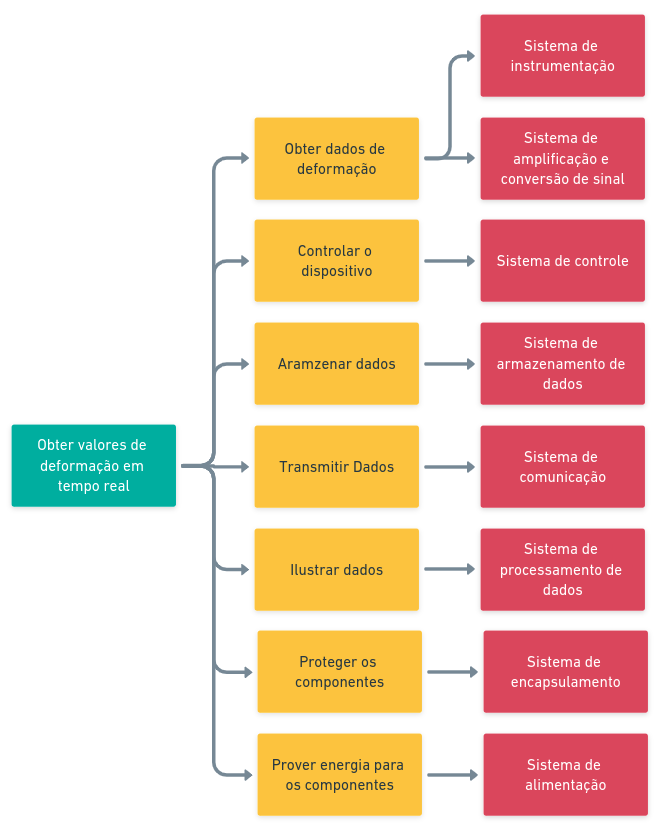
\includegraphics[width=350]{pictures/2031.png}
	\end{center}
	\fonte{O autor 2022}
\end{figure}

A partir da análise da matriz de listagem de atributos e da pesquisa com o público alvo é feito um levantamento das principais características do produto final:

\begin{alineas}

	\item Preço final
	\item Capacidade de processamento
	\item Taxa de obtenção de dados
	\item Sistema de armazenamento
	\item Software com interface gráfica
	\item Comunicação sem fio
	\item Capacidade da bateria
	\item Diâmetro da carcaça
	\item Comprimento da carcaça
	\item Sistema de vedação
	\item Sistema de resistência a impactos
	\item Massa total

\end{alineas}

Com os dados de avaliação quantitativa dos requisitos do produto obtidos pela pesquisa com o público alvo e os dados das características do produto é elaborada uma matriz de  avaliação de qualidade, ou QFD.
Essa matriz serve para correlacionar os requisitos com as características desejadas do produto, com a finalidade de apontar quais as qualidades devem ser priorizadas na etapa de desenvolvimento do projeto.
Os símbolos preenchidos na matriz qfd representam os fatores de correlação, que numericamente são iguais a 9 para correlação forte, 3 para correlação média e 1 para correlação fraca.

\begin{figure}[htb]
	\caption{\label{fig:2032} Matriz QFD}
	\begin{center}
		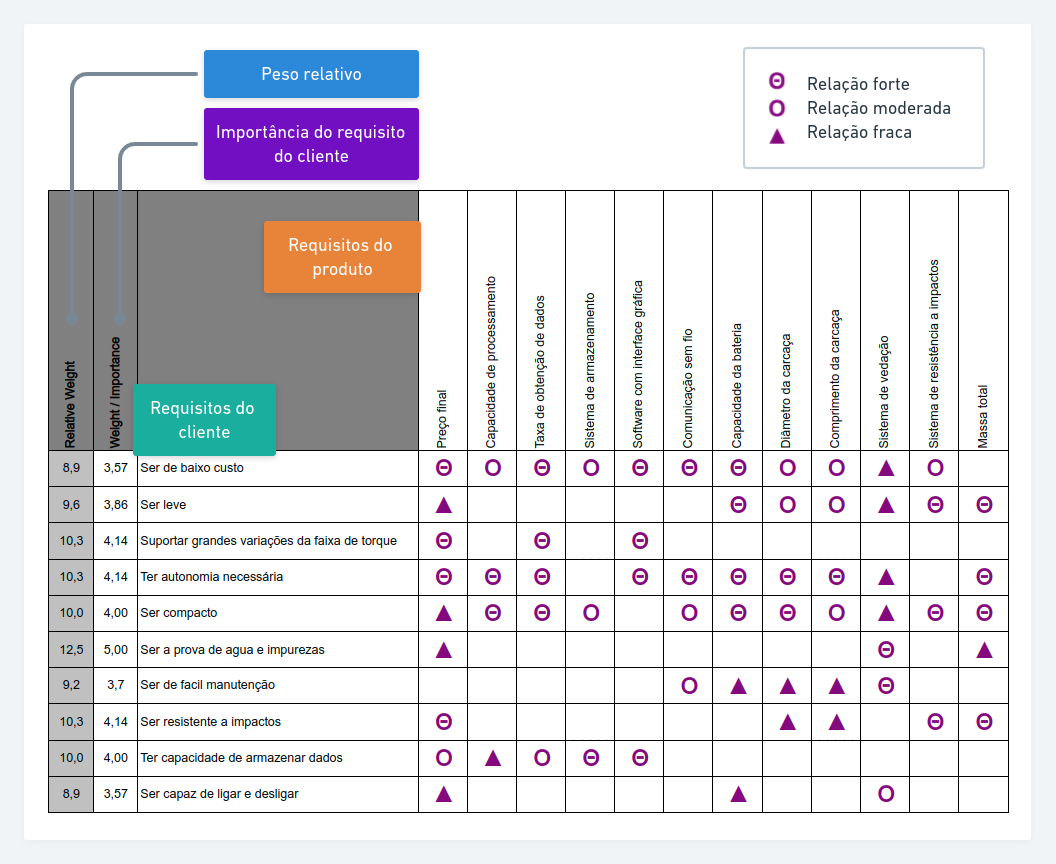
\includegraphics[width=\textwidth]{pictures/2032.png}
	\end{center}
	\fonte{O autor 2022}
\end{figure}

Os resultados de peso de importância para cada requisito de qualidade é calculado pelo somatório das multiplicações entre fator de correlação e o peso relativo relativos dos requisitos do cliente.
Os resultados de priorização obtidos pela matriz QFD são apresentados na \autoref{tab:resultqfd}.

\begin{table}[H]
    \caption{Prioridade dos requisitos definidos pela matriz QFD}
    \label{tab:resultqfd}
    \centering
    \resizebox{\textwidth}{!}{%
        \begin{tabular}{ l | c r } \toprule
			Característica 						& 	Peso de importância 	& Prioridade \\
			\midrule
			Preço Final							& 	429,5 					& alta \\
			Capacidade de processamento 		& 	219,2 					& baixa \\
			Taxa de obtenção de dados 			& 	385,4 					& média \\
			Sistema de armazenamento 			& 	146,3 					& baixa \\
			Software com interface gráfica 		& 	355,5 					& média \\
			Comunicação sem fio 				& 	230,6 					& baixa \\
			Capacidade da bateria 				& 	367,3 					& média \\
			Diâmetro da carcaça 				& 	257,7 					& baixa \\
			Comprimento da carcaça 				& 	197,9 					& baixa \\
			Sistema de vedação 					& 	260,8 					& baixa \\
			Sistema de resistência a impactos 	& 	295,8 					& baixa \\
			Massa total 						& 	374,4 					& média \\
            \bottomrule
        \end{tabular}}
\fonte{O autor 2022}\
\end{table}

A priorização dos requisitos é utilizado para guiar a tomada de decisões de projeto e escolha de componentes nos estágios do projeto conceitual.

\section{Projeto conceitual}

Na fase de projeto conceitual são avaliadas tecnicamente e economicamente as alternativas levantadas para se desenvolver um dispositivo que atenda os requisitos de cliente e de projeto.
O conceito de funcionamento básico do dispositivo é ilustrado na \autoref{fig:2035}.

\begin{figure}[H]
	\caption{\label{fig:2035} Conceito de funcionamento inicial}
	\begin{center}
		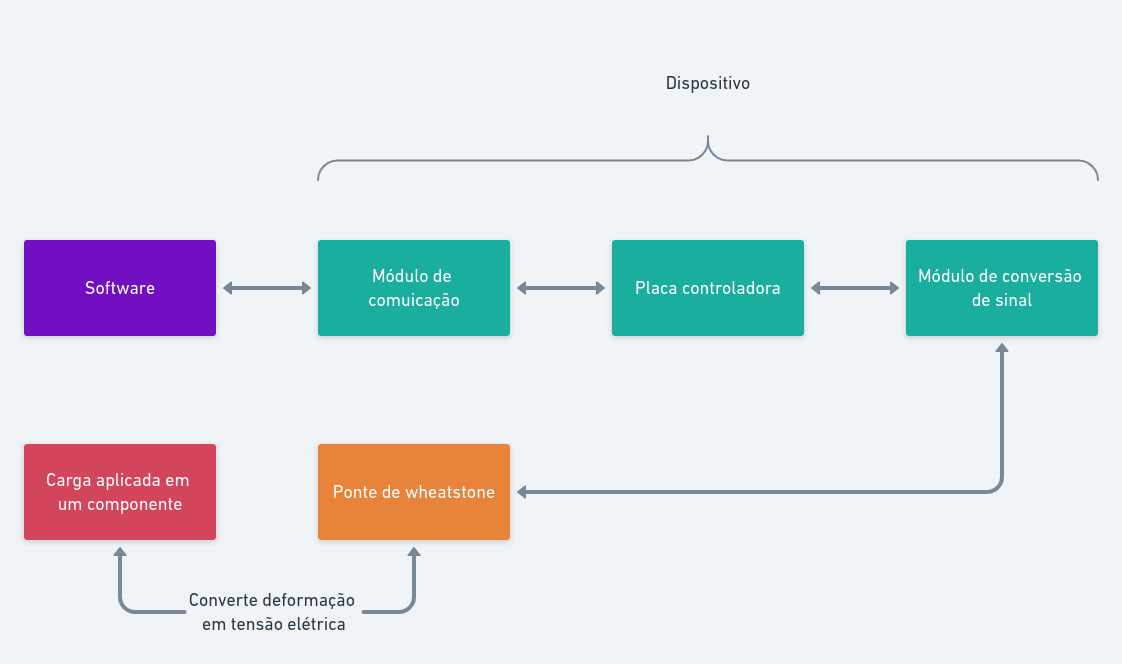
\includegraphics[width=\textwidth]{pictures/2035.png}
	\end{center}
	\fonte{O autor 2022}
\end{figure}

As opções de placa controladora avaliadas foram o Arduino Nano, o ESP32 ou o ESP8266, todos podem ser programados utilizando a linguagem de programação Arduino, e podem ser
encontrados por preços menores que 60 reais, as principais diferenças entre os controladores são de que os módulos ESP possuem opções de comunicação sem fio integradas.

Caso seja necessária a utilização de comunicação sem fio em um módulo que não possua integrado as principais opções disponíveis são o módulo bluetooth HC-05, que tem o custo
aproximado de 50 reais e o módulo wifi ESP8266, que tem o custo aproximado de 25 reais.
A comunicação bluetooth funciona com a transferência de dados diretamente entre o módulo e o receptor.
E a comunicação wifi pode ser feita tanto pela conexão do dispositivo receptor diretamente ao módulo bluetooth quanto pela comunicação entre servidor e cliente.

As opções de módulo de amplificação de sinal avaliadas foram o HX711, que se apresenta como um módulo altamente utilizado em aplicações de células de carga porém apresenta
uma taxa de leitura baixa, de até 80 amostras por segundo, e o ADS1115, que possui diversas opções de fator de amplificação que podem ser programadas e uma taxa de amostragem de 860 amostras
por segundo.
Ambos os módulos de amplificação já possuem conversores ADC integrados.

Apenas uma solução foi considerada como adequada para armazenamento de dados locais pelo dispositivo, que é a utilização de um módulo de cartão Micro SD, devido ás baixas dimensões.
Também foram avaliadas opções de alimentação energética para o dispositivo, materiais para construção do encapsulamento externo.
Uma breve apresentação do levantamento de componentes é mostrado na \autoref{tab:levantamentocomponentes}.

\begin{table}[!ht]
    \caption{Levantamento de componentes}
    \label{tab:levantamentocomponentes}
    \centering
    \resizebox{\textwidth}{!}{%
        \begin{tabular}{ l c r } \toprule
		Tipo de componente & Características principais & Preço aproximado \\
		\midrule
		\multicolumn{1}{l}{\textbf{Controladores}} & \\
			Arduino nano & compacto e fácil de programar & $R\${60.00}$ \\
			ESP 32 & comunicação sem fio integrada & $R\${40.00}$ \\
		\multicolumn{1}{l}{\textbf{Amplificadores de sinal}} & \\
			HX711 & Desenvolvido para aplicações de célula de carga & $R\${20.00}$ \\
			ADS1115 & Alta taxa de leitura & $R\${70.00}$ \\
			LM358 & Alta taxa de ganho & $R\${10.00}$ \\
		\multicolumn{1}{l}{\textbf{Comunicação sem fio}} & \\
			Bluetooth HC-05 & Difícil programação, emite e recebe dados  & $R\${50.00}$ \\
			Módulo wifi & Fácil acesso a qualquer dispositivo na mesma rede & $R\${25.00}$ \\
			Módulo radiofrequência & Comunicação apenas do transmissor para o receptor & $R\${15.00}$ \\
		\multicolumn{1}{l}{\textbf{Armazenamento}} & \\
			Módulo cartão micro SD + cartão SD & Permite armazenamento de dados & $R\${30.00}$ \\
		\multicolumn{1}{l}{\textbf{Alimentação}} & \\
			4x pilha AAA & mais compacto, alta disponibilidade & $R\${30.00}$ \\
			1x Bateria 9V & alta tensão e duração & $R\${40.00}$ \\
			2x Bateria li-ion & grandes dimensões, recarregável & $R\${35.00}$ \\
		\multicolumn{1}{l}{\textbf{Encapsulamento}} & \\
			Carcaça ABS & Pode fabricado por impressão 3D & -- \\
			Carcaça multi material & Maior custo com fabricação, maior resistência & -- \\
            \bottomrule
        \end{tabular}}
\fonte{O autor 2022}\
\end{table}

Após feito o levantamento de componentes pode-se montar a matriz morfológica, que serve para relacionar cada função elementar principal originada da matriz de
funções do produto com os componentes levantados anteriormente.
A matriz morfológica é mostrada na \autoref{fig:2036}.

\begin{figure}[H]
	\caption{\label{fig:2036} Matriz morfológica}
	\begin{center}
		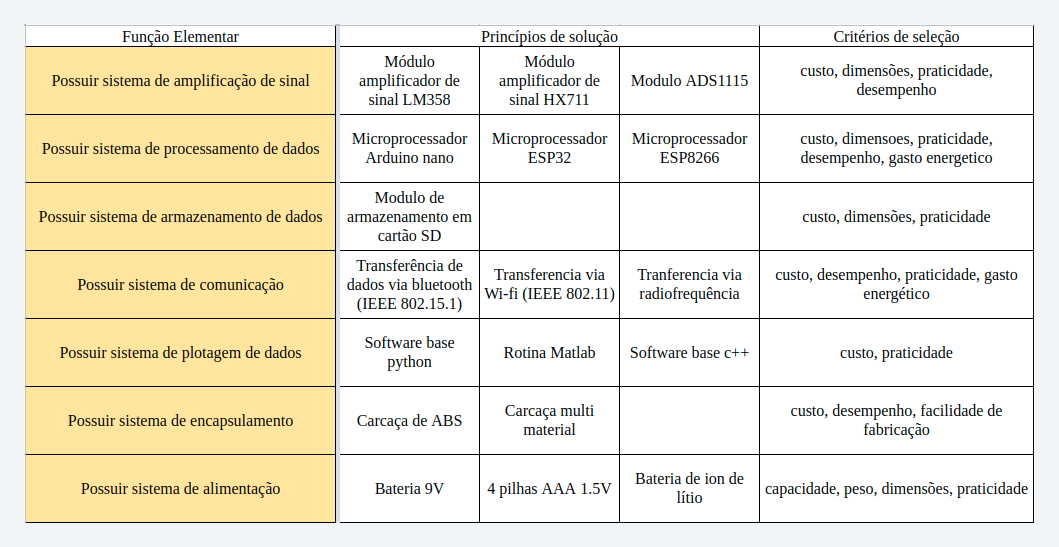
\includegraphics[width=\textwidth]{pictures/2036.png}
	\end{center}
	\fonte{O autor 2022}
\end{figure}

Na matriz morfológica também foi adicionado uma coluna para listar os principais requisitos de avaliação de cada produto, esses requisitos mostrados estão diretamente
relacionados com os requisitos de cliente e produto obtidos da análise da matriz da casa da qualidade.
Para a avaliação e comparação das soluções em relação aos requisitos levantados é utilizado a matriz de avaliação, mostrada na \autoref{fig:2037} a matriz de avaliação
lista as possíveis tecnologias utilizadas para a solução e os requisitos, e para cada relação uma nota de comparação é definida entre -3, que significa que a tecnologia
é a mais adequada ao requisito relacionado, até 3, que significa que a tecnologia é a menos adequada ao requisito relacionado.

\begin{figure}[H]
	\caption{\label{fig:2037} Matriz de avaliação}
	\begin{center}
		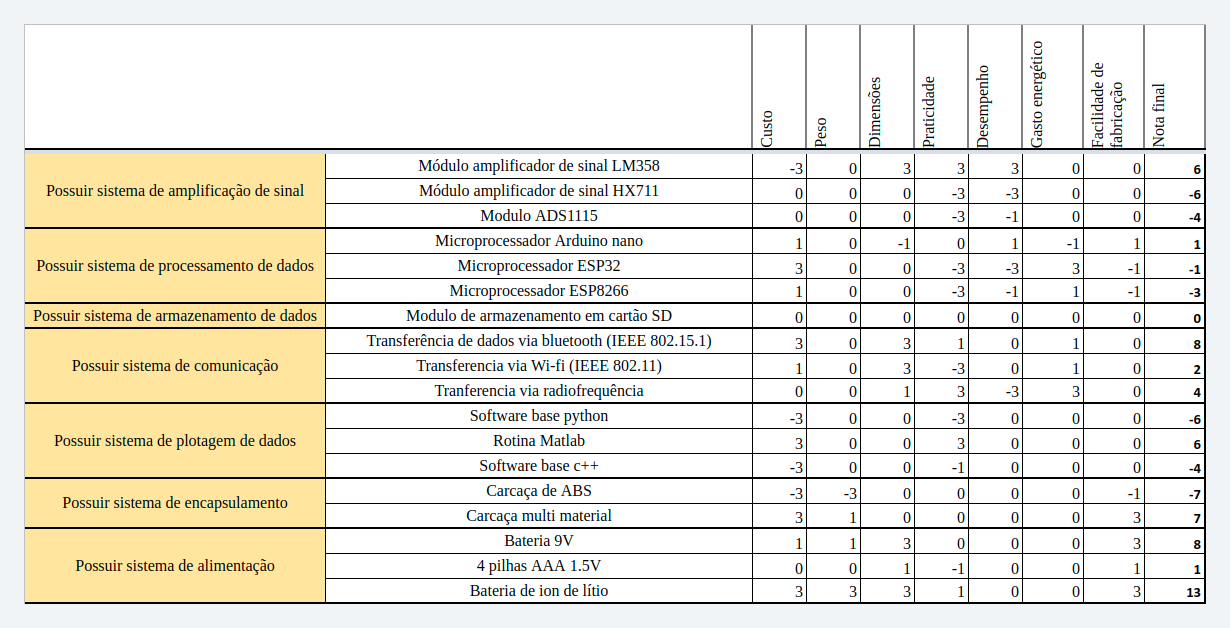
\includegraphics[width=\textwidth]{pictures/2037.png}
	\end{center}
	\fonte{O autor 2022}
\end{figure}

A matriz de avaliação resulta em um valor quantitativo que avalia o quão adequado cada opção tecnológica é ao projeto do dispositivo.
Após a análise dos resultados da matriz de avaliação as tecnologias escolhidas são mostradas na \autoref{fig:2038}.

\begin{figure}[H]
	\caption{\label{fig:2038} Soluções escolhidas}
	\begin{center}
		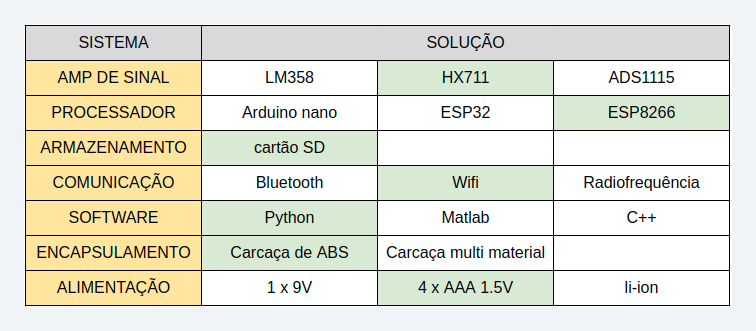
\includegraphics[width=\textwidth]{pictures/2038.png}
	\end{center}
	\fonte{O autor 2022}
\end{figure}

Após definido as tecnologias que serão utilizadas no desenvolvimento do produto, deve-se seguir para a etapa de projeto detalhado.

\section{Projeto detalhado}

A documentação do projeto detalhado do produto é composta pelos projetos mecânico, elétrico/eletrônico e pelo desenvolvimento do software de comunicação.

O projeto mecânico do dispositivo foi desenvolvido utilizando o software Solidworks 2017, os modelos da placa de controle ESP8266 e do amplificador de sinal HX711
foram obtidos na plataforma de compartilhamento de modelos GrabCAD. Após ser definido um arranjo inicial da posição dos componentes no dispositivo foi modelado um
componente de encapsulamento para o dispositivo.
O modelo da montagem do dispositivo é ilustrado na \autoref{fig:2039}.

\begin{figure}[H]
	\caption{\label{fig:2039} Modelagem da montagem do dispositivo}
	\begin{center}
		\includegraphics[width=\textwidth]{pictures/2039.png}
	\end{center}
	\fonte{O autor 2022}
\end{figure}

A ilustração do projeto do dispositivo nas três vistas padrão e vista isométrica é mostrado na \autoref{fig:2040}.

\begin{figure}[H]
	\caption{\label{fig:2040} Desenho em vistas padrões (primeiro diedro)}
	\begin{center}
		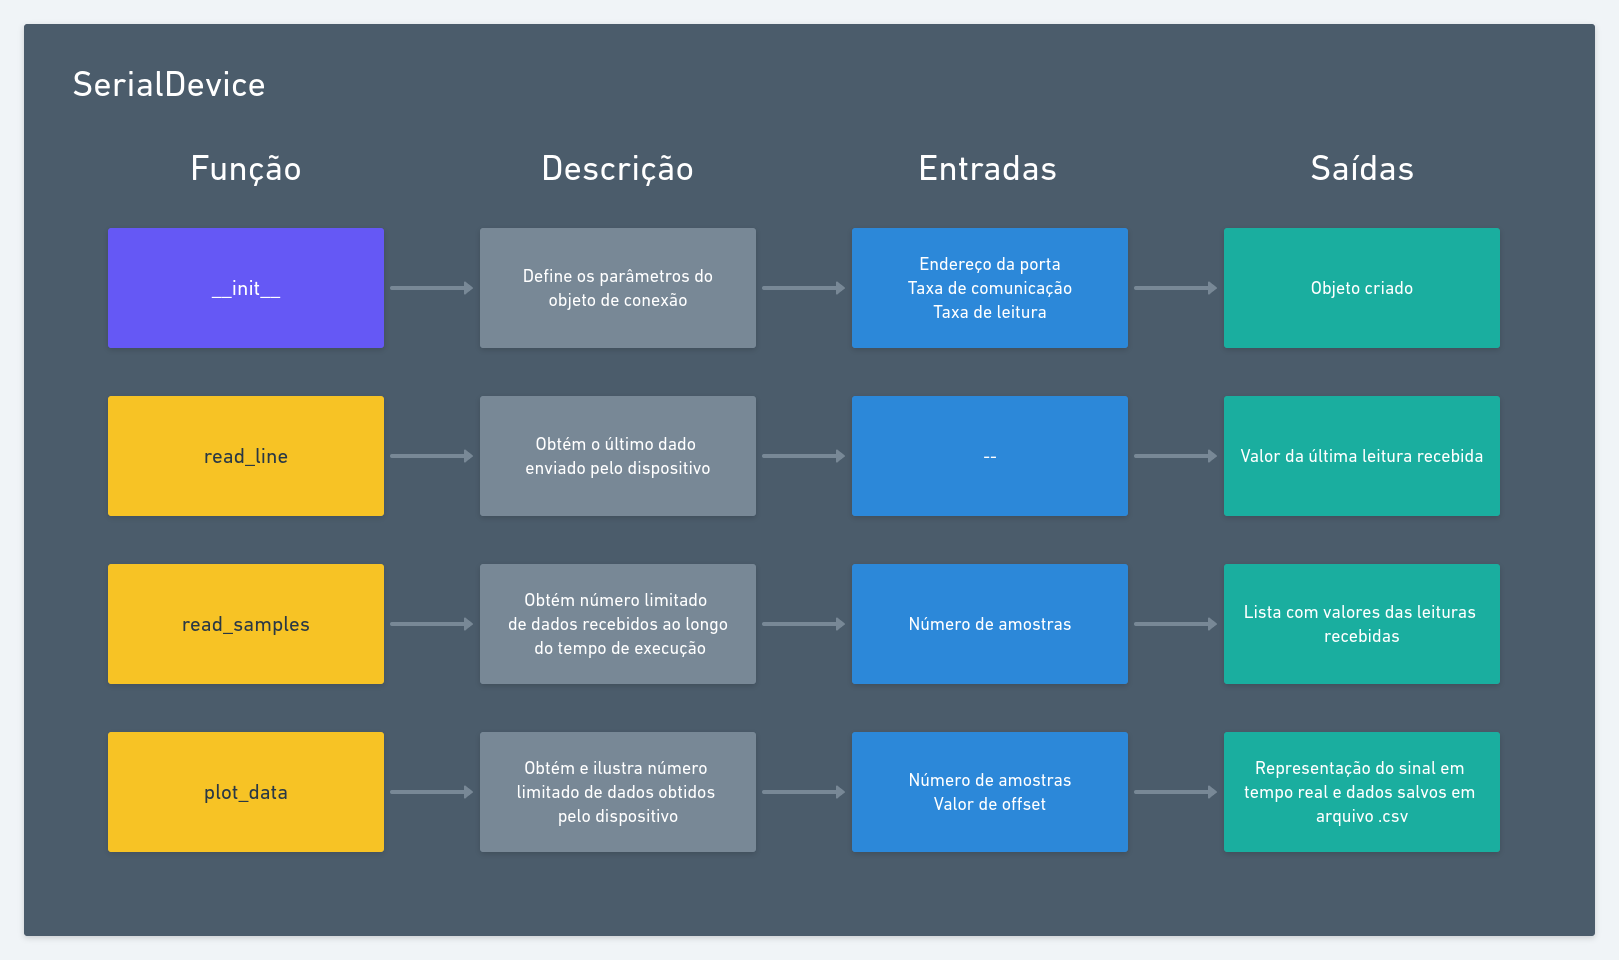
\includegraphics[width=\textwidth]{pictures/2040.png}
	\end{center}
	\fonte{O autor 2022}
\end{figure}

O projeto elétrico do dispositivo foi desenvolvido utilizando o software para desenvolvimento de placas eletrônicas EasyEDA e é mostrado na \autoref{fig:2041}.

\begin{figure}[H]
	\caption{\label{fig:2041} Projeto elétrico do dispositivo}
	\begin{center}
		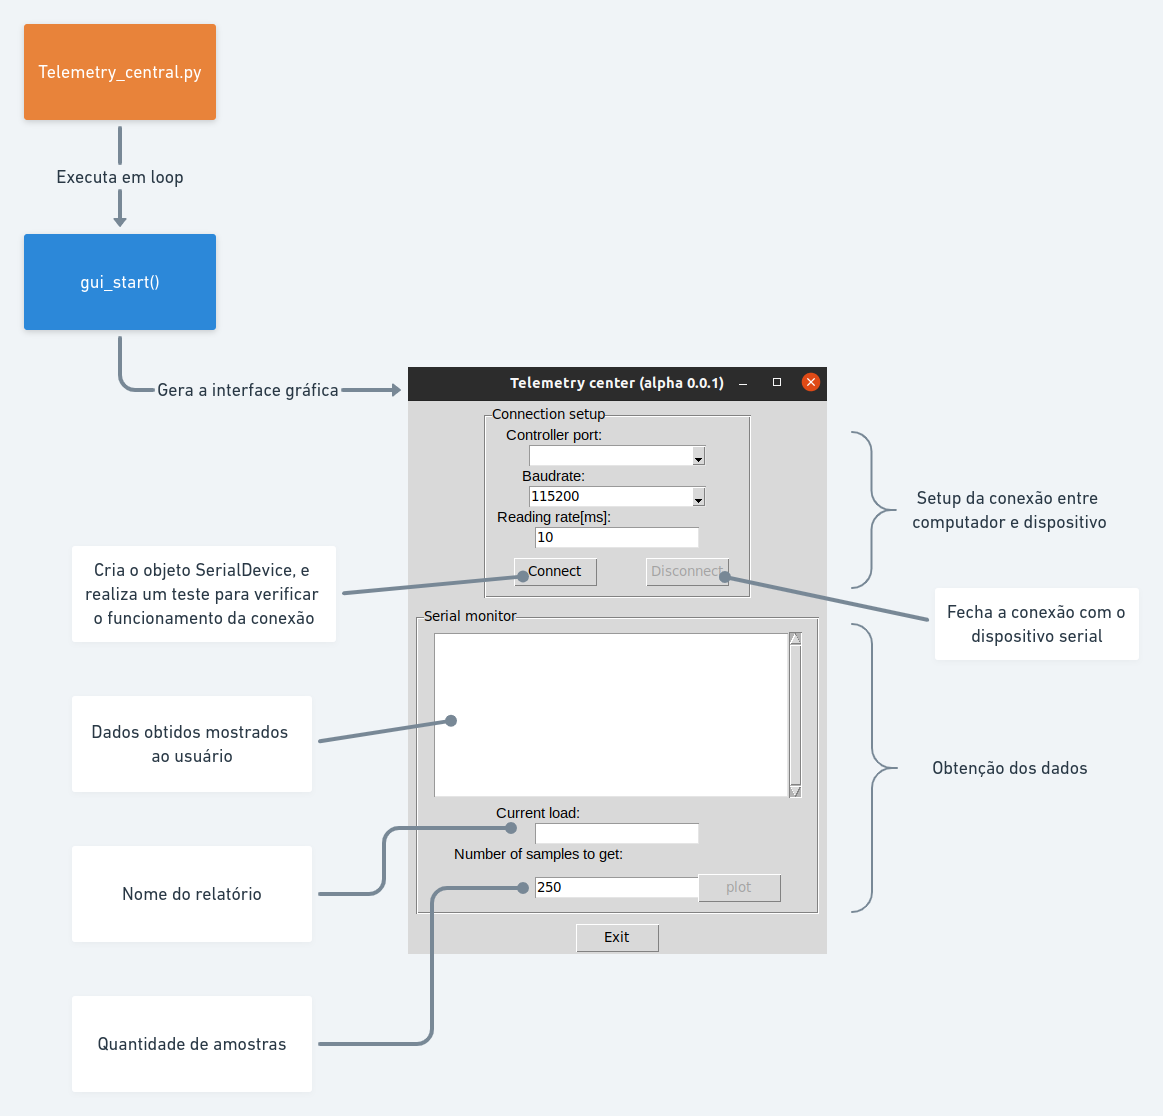
\includegraphics[width=\textwidth]{pictures/2041.png}
	\end{center}
	\fonte{O autor 2022}
\end{figure}

A fase de desenvolvimento do software engloba duas etapas principais, a primeira é o desenvolvimento da programação da placa de controle,
que é feita utilizando o programa Arduino IDE para conectar e programar o controlador da plataforma.
Uma introdução a estrutura do programa de controle e das suas funções é mostrada na \autoref{fig:2042}

\begin{figure}[H]
	\caption{\label{fig:2042} Esquema da programação do dispositivo}
	\begin{center}
		\includegraphics[width=\textwidth]{pictures/2042.png}
	\end{center}
	\fonte{O autor 2022}
\end{figure}

A programação da placa de controle é feita com uma linguagem de programação baseada em C++, com funções específicas para a programação de controladores de
plataformas abertas, como o Arduino e o ESP8266.

A função handleRead utiliza o método hx711.read(), conforme o \autoref{lst:handle_read}, para obter os valores de tensão na saída da ponte de wheatstone e os
enviar ao computador via rede local.
O programa completo do controlador completo é apresentado no \autoref{ch:algoritmo-de-programação-do-controlador-do-dispositivo}.

\begin{lstlisting}[label={lst:handle_read},language=C++,caption={[Controller Program]{Função de obtenção de sinal pelo amplificador HX711}}]

void handleRead() {
  if (server.method() != HTTP_POST) {
    server.send(405, "text/plain", "Method not allowed");
  } else {
    server.send(200, "text/plain", String(hx711.read()) + server.arg("plain"));
  }
}

\end{lstlisting}

Uma vez configurado o controlador do dispositivo, foi desenvolvido utilizando a linguagem Python um objeto computacional para facilitar a conexão e utilização dos dados originados pelo dispositivo.
O objeto e suas funções é ilustrado pela \autoref{fig:2043}.

\begin{figure}[htb]
	\caption{\label{fig:2043} Objeto NetworkDevice}
	\begin{center}
		\includegraphics[width=\textwidth]{pictures/2043.png}
	\end{center}
	\fonte{O autor 2022}
\end{figure}

As funções de base do objeto são mostradas na \autoref{lst:essentialobjectfuncions}.
O método \_\_init\_\_ recebe e salva como parâmetros do objeto os dados de endereço de ip do dispositivo e intervalo de leitura inseridos,
e o método read\_line utiliza a função post do pacote requests para enviar uma requisição ao endereço de ip do objeto e retorna o valor obtido em forma de
texto de maneira calibrada, caso o argumento calibrated seja igual a verdadeiro, ou não calibrado, caso contrário.

\begin{lstlisting}[label={lst:essentialobjectfuncions},language=Python,caption={[NetworkDevice]{Métodos base do objeto NetworkDevice}}]

"""
Creates a local network connection device object
"""

def __init__(self, ip, delay_time):
	self.url = f'http://{ip}/read'
	self.delay_time = delay_time
	self.offset = 0
	self.a = 1
	self.b = 0

def read_line(self, calibrated: bool = False):
	"""returns the last line of data sent by the device"""
	read = int(post(self.url).text) - self.offset
	if calibrated:
		return self.a * read + self.b
	else:
		return read

\end{lstlisting}

Caso seja necessária a obtenção de dados em sequência ao longo do tempo foram desenvolvidas as funções read\_samples e plot, mostradas na \autoref{lst:sample_reading},
o número de amostras é passado para a obtenção repetida dos dados, utilizando o parâmetro de intervalo de leitura para determinar o intervalo de execução da chamada do
método read\_line, e é retornado um objeto de lista do Numpy com os dados obtidos.

\begin{lstlisting}[language=Python,label={lst:sample_reading},caption={[Network Device calibrate offset]{Métodos para executar experimentos do objeto NetworkDevice}}]

def read_samples(self, n_of_samples: int, plot: bool = False, calibrated: bool = False):
	"""returns a number of data lines given a sample size"""

	if not plot:
		value_list = array([])
		while len(value_list) < n_of_samples:
			value_list = append(
				value_list,
				int(self.read_line(calibrated=calibrated))
			)
			sleep(self.delay_time)

	else:
		value_list = self.plot_data(n_of_samples=n_of_samples, calibrated=calibrated)

	return value_list

def plot_data(self, n_of_samples: int, calibrated: bool = False):
	"""plot the numerical data received"""
	value_list = array([])

	plt.ion()
	fig, axs = plt.subplots(1)
	fig.suptitle('Readings')

	while len(value_list) < n_of_samples:
		try:
			value_list = append(value_list, int(self.read_line(calibrated=calibrated)))

			axs.cla()
			axs.plot(value_list[-25:])

			plt.pause(self.delay_time)

		except:
			print("error!")

	plt.close()

	return value_list

\end{lstlisting}

As funções de calibração do objeto de conexão com o dispositivo são mostradas no \autoref{lst:objectcalibration}. O método calibrate\_offset serve para definir o ponto de leitura quando
nenhuma carga está presente, e funciona obtendo 40 amostras utilizando o método read\_samples, arredondando o valor médio dessas amostras a um número inteiro e definindo o parâmetro
offset do objeto ao valor obtido. A função calibrate readings utiliza recebe duas cargas nominais conhecidas e seus sinais obtidos em forma de dicionário e utiliza estes valores para
definir os parâmetros a e b da função linear de calibração, com a finalidade de ser utilizada no método read\_line para converter os valores em forma de bits para um formato de valor
nominal da grandeza física calibrada.

\begin{lstlisting}[label={lst:objectcalibration},language=Python,caption={[Network Device calibrate offset]{Métodos de calibração do objeto NetworkDevice}}]

def calibrate_offset(self):
	"""sets the offset value for the device data gathering"""
	self.offset = 0
	self.offset = round(self.read_samples(n_of_samples=40).mean())

def calibrate_readings(self, calibration_dict_1: dict, calibration_dict_2: dict):
	"""calibrate the device readings"""
	w1 = calibration_dict_1['nominal_value']
	w2 = calibration_dict_2['nominal_value']
	r1 = round(calibration_dict_1['signal'].mean())
	r2 = round(calibration_dict_1['signal'].mean())

	self.b = w2 / ((r2 / r1) * (w1 - 1) + 1)
	self.a = (w1 - self.b) / r1

\end{lstlisting}

Com o intuito de facilitar a utilização do método pelo usuário é desenvolvido uma interface gráfica simples, uma breve apresentação da interface desenvolvida utilizando o pacote tkinter é mostrada na \autoref{fig:2044}.

\begin{figure}[H]
	\caption{\label{fig:2044} Interface gráfica}
		\begin{center}
			\includegraphics[width=\textwidth]{pictures/2044.png}
		\end{center}
	\fonte{O autor 2022}
\end{figure}

Os códigos completos para o objeto NetworkDevice e para a geração da interface gráfica são apresentados no \autoref{ch:algoritmos-desenvolvidos-para-o-software-de-conexão}.

\section{Validação do protótipo do dispositivo}

Após a conclusão da fase de projeto detalhado foi montado o protótipo do dispositivo, com a finalidade ser executar experimentos de validação. O dispositivo montado é mostrado na \autoref{fig:2045}

\begin{figure}[H]
	\caption{\label{fig:2045} Protótipo preparado para os experimentos}
		\begin{center}
			\includegraphics[width=\textwidth]{pictures/2045.png}
		\end{center}
	\fonte{O autor 2022}
\end{figure}

A metodologia de execução do experimento para validar o funcionamento do protótipo desenvolvido segue a mesma metodologia do experimento realizado no trabalho de conclusão
de curso de \autocite{Minela2017}, uma introdução aos principais tópicos dessa metodologia e eventuais diferenças entre os dispositivos utilizados nos dois trabalhos para cada tópico é feita nessa seção.

Os ensaios realizados envolvem a leitura de extensômetros colados em corpos de prova sobre ação de cargas específicas. Um dispositivo de análise de cargas de flexão e
um para cargas em torção foram desenvolvidos e produzidos por \autocite{Minela2017}, os mesmos dispositivos foram utilizados para este trabalho.

\subsection{Dispositivo para ensaio de flexão}

O dispositivo para realizar o ensaio de flexão é composto por uma viga de seção retangular de $20mm$ de largura por $2mm$ de espessura, que mede $200mm$
de comprimento e é de uma liga desconhecida de alumínio, e uma base projetada e fabricada em aço 1020 para fixar a viga em uma situação de engaste na viga.
A imagem mostra o projeto do dispositivo desenvolvido por \autocite{Minela2017}.

\begin{figure}[htb]
	\caption{\label{fig:2049} Dispositivo de ensaio de flexão}
	\begin{center}
		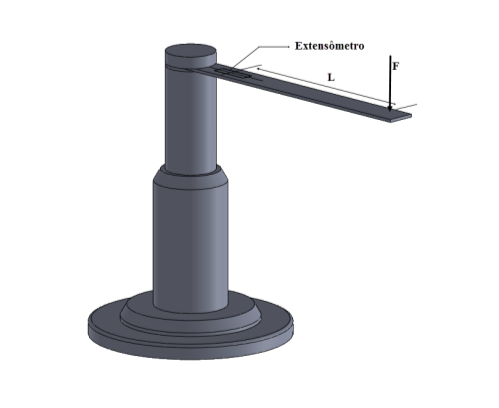
\includegraphics[width=\textwidth]{pictures/2049.png}
	\end{center}
	\fonte{\autocite{Minela2017}}
\end{figure}

Na viga é colado um extensômetro unidimensional para obter os dados de deformação, as propriedades do extensômetro utilizado são mostradas na
\autoref{tab:PropriedadesExtensometro}.

\begin{table}[htb]
\caption[]{Propriedades do extensômetro colado ao dispositivo de flexão}
\label{tab:PropriedadesExtensometro}
\resizebox{\textwidth}{!}{%
\begin{tabular}{p{6.5cm}p{8cm}}
	\toprule
	Marca & Micro Measurements \textregistered \\
	Tipo de extensômetro & EA-06-250AF-120 \\
	Resistência Elétrica & ${120\pm 0.15\% \Omega}$ \\
	Factor de gage até ${75 ^\circ F}$ & ${2.025 \pm 0.5 \%}$ \\
	Comprimento & ${6.35} \mm$ \\
	Limite de têmperatura & ${-75\tccentigrade}$ á ${175\tccentigrade}$ para medições estáticas \\
	\bottomrule
\end{tabular}
}
\fonte{Adapdato de \autocite{Minela2017}}
\end{table}

As cargas são aplicadas na extremidade livre da viga a distância de 150mm entre o centro do extensômetro e o ponto de aplicação da carga.
Com a finalidade de se obter os valores de deformação causados pela aplicação de cada carga, cada trabalho utiliza-se de um sistema de medição diferente, apresentado
na seção seguinte.

\subsection{Sistemas de medição}

Tanto o sistema de medição utilizado em \autocite{Minela2017} quanto o utilizado para o desenvolvimento deste trabalho seguem o mesmo princípio de funcionamento.

\begin{figure}[htb]
	\caption{\label{fig:2050} Sistema de medição utilizado por \autocite{Minela2017}}
	\begin{center}
		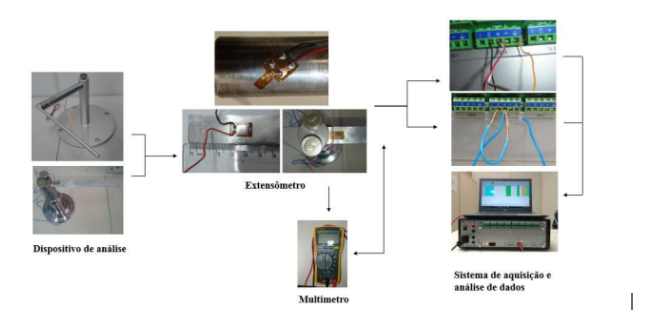
\includegraphics[width=\textwidth]{pictures/2050.png}
	\end{center}
	\fonte{\autocite{Minela2017}}
\end{figure}

O sistema de medição utilizado por \autocite{Minela2017} é composto por um dispositivo de obtenção de dados ADS2002, desenvolvido e fabricado pela LYNX Tecnologia,
que é conectado a um computador. O ADS2002 obtém os dados gerados pelo sensor e os envia ao computador via conexão ethernet.
O computador utiliza o software AQDados para conexão com o ADS2002, calibração e aferição dos extensômetros, e o softwre AqAnalysis para fazer o processamento dos sinais
e gerar relatórios de análise, ambos os programas são desenvolvidos pela fabricante do dispositivo de obtenção de dados.

\begin{figure}[htb]
	\caption{\label{fig:2060} Sistema de de medição utilizando o LINX ADS2002}
	\begin{center}
		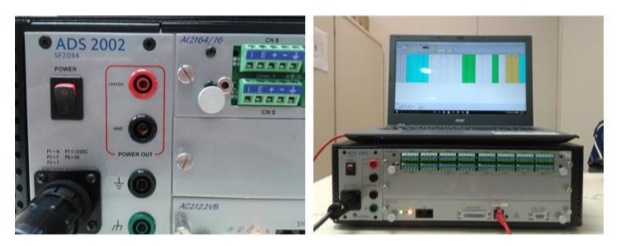
\includegraphics[width=\textwidth]{pictures/2060.png}
	\end{center}
	\fonte{\autocite{Minela2017}}
\end{figure}

A conexão entre o dispositivo de obtenção de dados e o extensômetro ocorre utilizando os terminais elétricos do canal específico de análise, o ADS2002 já possui,
integrado em si, os componentes elétricos do circuito da ponte de wheatstone para a instrumentação do sinal.
A calibração do extensômetro afim dos resultados serem mostrados como valores deformação, ao invés de tensões, é feita utilizando a \autoref{eq:Eq_270} que define um valor de
fator de engenharia em função do fator gage $FG$ da resistência média do extensômetro $RM$, resistência de calibração $RC$, que é disponibilizada pelo fabricante.

\begin{equation}\label{eq:Eq_270}%
\mbox{\fontsize{17.28}{21.6}\selectfont\( %
VE = \left ( \frac{1}{FG}\left ( \frac{RM}{RM + RC} \right ) \right )
\)} %
\end{equation}

\newline

O sistema de medição utilizando o protótipo desenvolvido pelo autor é feito pela conexão entre o controlador ESP 32 e o computador via o software desenvolvido em Python
para realizar a transferência dos dados obtidos entre o controlador e o computador em tempo real.

\begin{figure}[htb]
	\caption{\label{fig:2070} Protótipo do dispositivo desenvolvido conectado com o extensometro no dispositivo de flexão}
	\begin{center}
		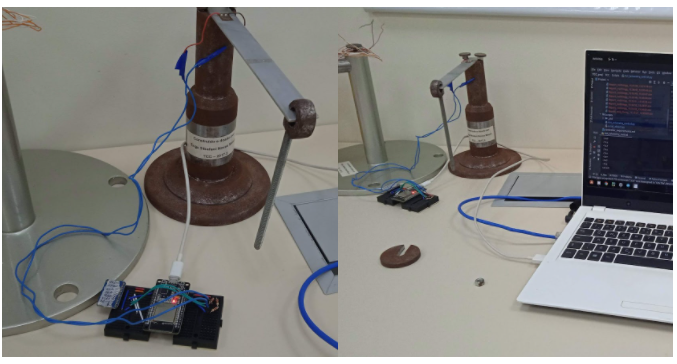
\includegraphics[width=\textwidth]{pictures/2070.png}
	\end{center}
	\fonte{O autor 2021}
\end{figure}

A calibração do dispositivo desenvolvido pelo autor é feita utilizando os sinais resultantes da aplicação de duas massas distintas conhecidas.
Os valores nominais obtidos nos sinais alimentam a \autoref{eq:Eq_280} que é utilizada para converter os valores discretos obtidos em bits pelo
amplificador de sinal para um valor de gradeza física desejado.

\begin{equation}\label{eq:Eq_280}%
\mbox{\fontsize{17.28}{21.6}\selectfont\( %
F(W) = \frac{output_{high}-output_{low}}{W_{high}-W_{low}}(W - W_{low}) + output_{low}
\)} %
\end{equation}

%onde
%
%$F(W)$: Função de calibração
%
%$W$: Valor nominal do sinal
%
%$W_{high}$: Carga de calibração de massa alta
%
%$W_{low}$: Carga de calibração de massa baixa
%
%$output_{high}$: Valor nominal do sinal obtido pela aplicação da carga alta
%
%$output_{high}$: Valor nominal do sinal obtido pela aplicação da carga baixa

\hfill

A calibração ocorre por um método automatizado implementado no software de comunicação entre o controlador e o computador.
Após calibrado, o dados são mostrados como os valores de grandeza física calibrada.

\subsection{Cargas aplicadas}

\autocite{Minela2017} utiliza pesos com massas pré definidas apoiadas utilizando um fuso de fixação para aplicação das cargas no ponto “F” no dispositivo, mostrado na figura.
Dentre as massas utilizadas por \autocite{Minela2017} duas não foram localizadas pelo autor deste trabalho, com a finalidade de poder se obter resultados que se possam fazer
comparações diretas entre os trabalhos foram substituídas as massas não encontradas por massas semelhantes.

Todos os valores de massa dos pesos utilizados foram obtidos novamente pelo autor utilizando o valor médio de três leituras obtidas por uma balança de precisão disponibilizada pelo laboratório de metrologia
da UFSC Joinville. Os valores obtidos são apresentados na \autoref{tab:MassasUtilizadas}.

\begin{table}[!ht]
    \caption{Valores de massas utilizadas para aplicação das cargas nos dispositivos de flexão e torção}
    \label{tab:MassasUtilizadas}
    \centering
    \resizebox{\linewidth}{!}$ \\
            Fuso & $\SI{48.63}{\g}$ & $\SI{48.78}{\g}$ & $\SI{0.31}{\%}$ \\
            Peso 1 & $\SI{86.73}{\g}$ & $\SI{99.68}{\g}$ & $\SI{12.99}{\%}$ \\
            Peso 2 & $\SI{198.38}{\g}$ & $\SI{198.36}{\g}$ & $\SI{0.01}{\%}$ \\
            Peso 3 & $\SI{997.13}{\g}$ & $\SI{997.3}{\g}$ & $\SI{0.02}{\%}$ \\
            Peso 4 & $\SI{497.66}{\g}$ &$\SI{497.69}{\g}$ & $\SI{0.02}{\%}$ \\
            Peso 5 & $\SI{495.25}{\g}$ & $\SI{496.22}{\g}$ & $\SI{0.20}{\%}$ \\
            \bottomrule
        \end{tabular}}
\fonte{O autor 2022}
\end{table}

As massas da porca e do “peso 1” utilizados em \autocite{Minela2017} variam de forma considerável em relação aos pesos utilizados neste trabalho, então para todas as comparações diretas de
resultados experimentais obtidos entre os dois trabalhos deve ser aplicados fatores de correção de 11.42g para a porca e 12.95g para o “peso 1”.

O método de aplicação de cargas é caracterizado pela aplicação na extremidade livre da viga das massas utilizando o fuso como suporte, a Figura mostra a viga de alumínio defletida pela aplicação da carga do "peso 3".

\begin{figure}[htb]
	\caption{\label{fig:2080} Aplicaçao do 'peso 3' no dispositivo de flexão}
	\begin{center}
		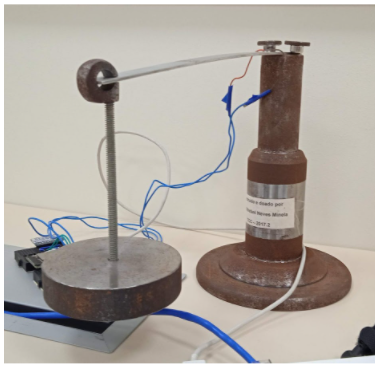
\includegraphics[width=\textwidth]{pictures/2080.png}
	\end{center}
	\fonte{O autor 2021}
\end{figure}

Na extremidade da viga encontra-se uma demarcação para auxiliar o posicionamento do apoio do fuso e as cargas são aplicadas de maneira cuidadosa de modo que não sejam geradas forças de impulso na viga.
O sistema de medição obtêm valores em bits proporcionais a carga aplicada no experimento.

Após a obtenção e armazenamento dos sinais obtidos nos experimentos prossegue-se para a etapa de análise dos resultados.
